\documentclass[a4paper, 11pt]{article}
\usepackage{comment} % enables the use of multi-line comments (\ifx \fi) 
\usepackage{fullpage} % changes the margin
\usepackage{hyperref}
\usepackage{mathtools}
\usepackage{amsmath}
\usepackage{booktabs} % For formal tables
\usepackage[ruled]{algorithm2e} % For algorithms
\renewcommand{\algorithmcfname}{ALGORITHM}
\DeclarePairedDelimiter{\ceil}{\lceil}{\rceil}


\begin{document}
\begin{titlepage}
   \begin{center}
       \vspace*{1cm}
 
       \textbf{\huge{SOEN 6011: SOFTWARE ENGINEERING PROCESSES}}
 
       \vspace{0.5cm}
        \textbf{\huge{Project Deliverable 1}}
 
       \vspace{1.0cm}
       \vskip 1.4in
    
\includegraphics[width=1.0\textwidth]{Concordia.jpg}
       
       \vskip 1.4in
 
       \vspace{0.8cm}
       
        \textbf{Himanshu Kohli}\\
        \textbf{Student Id : 40070839}\\
       Applied Computer Science\\
       Concordia University\\
       
 
   \end{center}
\end{titlepage}
\newpage
% @author : Himanshu Kohli
% Student ID: 40070839
% Date: 22 Feb 2019
\noindent
\large\textbf{Problem 1} \hfill \textbf{Himanshu Kohli} \\
\normalsize SOEN 6011 \hfill \textbf{40070839} \\
Prof. Pankaj Kamthan \hfill Due Date: July 19, 2019 \\


\section{Function 7 :  $a^{b^{x}}$}

The function $a^{b^{x}}$ is an exponential function where a and b are real constants and x is a real variable. A normal exponential function is stagnant at first but then increases sharply as the value of the variable increases. \\

The growth or decay of the function depends upon the sign of the exponent so if the sign is positive the function increases and if the sign is negative the function decreases.\\

for e.g. if x is positive the function : f(x) = $a^{b^{x}}$ \\

and if x is negative the function : f(x) = $\frac{1}{a^{b^{x}}}$ \\

The domain and co-domain of the function \\

If we differentiate the function with respect to x

\begin{equation} \label{eq. 1}
    \begin{split}
        \frac{d}{dx}  a^{b^{x}} & = a^{b^{x}} \log{a} * b^x \log{b}
    \end{split}
\end{equation} 
\newline
From equation \ref{eq. 1} we can see if the value of either a or b is equal to 1 the $\log{b}$ or $\log{a}$ equals to zero because $\log{1} = 0$ which means the exponential function is constant because the derivative is zero. \\
For a positive value of b and a the function $a^{b^{x}}$ is monotonically increasing \\
For a negative value of b and positive value of a the function $a^{b^{x}}$ is monotonically increasing in negative side i.e. (negative x axis)  \\
For a positive or negative value of b and negative value of a the function $a^{b^{x}}$ is monotonically decreasing  \\

So the value of the function f(x) = $a^{b^{x}}$ actually depends upon the $b^x$  and how the slope of the function will be rise or decay. \newline
Properties : 
\begin{enumerate}
    \item The domain is all real numbers
    \item The graph is continuous and smooth
    \item The graph can be asymptotic or increase without bounds
    \item The graph is monotonically increasing or decreasing
\end{enumerate}

\newpage

\section{Requirements Specifications}

\subsection{Introduction}
The implementation of well designed and well defined calculator function specifically $a^{b^{x}}$  falls in the range of exponential functions which gamuts to alpine values quickly. And within the function lies certain requirements which are to be fulfilled in order to make the entire system tangible.

\subsection{Requirements} 
\begin{enumerate}
    \item \textbf{Title :} Verifying input \newline 
    \textbf{Description : } The system should validate the of the inputs by the user where the variables a and b should be real constant and the x must be a real variable whereas any other values rather than real numbers should result in an error. \newline
    \textbf{Requirement Type : } Functional
    
    \item \textbf{Title :} Infinity representation \newline 
    \textbf{Description : } The system should have a calculation for infinity i.e. for specifically large numbers it should print the result as infinite. \newline
    \textbf{Requirement Type : } Functional, System
    
    \item \textbf{Title :} Input Domain \newline 
    \textbf{Description : } The system should perform operation on any numbers which falls under the domain of real numbers. \newline
    \textbf{Requirement Type : } Functional, Interface
    
    \item \textbf{Title :} Positive large number handling \newline 
    \textbf{Description : } The largest value java systems can handle is max double value of 1.8 * $10^{308}$ so if the function evaluation reaches max value it shall be considered as positive infinity. \newline
    \textbf{Requirement Type : } Functional, System
    
    \item \textbf{Title :} Negative large number handling \newline 
    \textbf{Description : } The lowest value java systems can handle is a min double value of 4.9 * $10^{-324}$ so if the function evaluation reach min value it shall be considered as negative infinity. \newline
    \textbf{Requirement Type : } Functional, System
    
    \item \textbf{Title :} Rounding input value \newline 
    \textbf{Description : } The system shall be able of handle decimal point numbers with a rounding of up to 10 decimal places for the inputs. \newline
    \textbf{Requirement Type : } Functional, Interface
    
    \item \textbf{Title :} Valid input and output \newline
    \textbf{Description : } The system shall take the input from command line and for a valid input it should print the valid result to the command line.
    \newline
    \textbf{Requirement Type : } Functional
    
    \item \textbf{Title :} Result Dependency on 'a' value \newline 
    \textbf{Description : } The function shall only print negative results when the value of a is negative and positive results when a is positive.
    
\end{enumerate}
\newpage
\section{Pseudo Code}
\subsection{Solution}
The function is $a^{b^x}$ can be solved using Taylor series and to do that I am breaking and converting the function into two parts which are: 
\begin{enumerate}
    \item Let y = $b^x$ which can be rewritten as $e^{x * log(b)}$
    \item And z = $a^y$ which can be rewritten as $e^{y * log(a)}$
\end{enumerate}
The normal Taylor series for 
\begin{equation} \label{exptaylor}
    e^x = 1 + \frac{x}{1!} + \frac{x^2}{2!}  + \frac{x^3}{3!} + \frac{x^4}{4!} ...... \frac{x^n}{n!}
\end{equation}
where n is the precision we are looking for. \newline
And we have to find the algorithm to find the log of a number which has a Taylor series of it's own. \newline
\begin{equation} \label{logtaylor}
\ln{\frac{1+x}{1-x}} = 2 * ( \frac{x}{1} + \frac{x^3}{3} + \frac{x^5}{5} + \frac{x^7}{7}  .....)
\end{equation}
\newline
So we have to implement two \textbf{subordinate} functions which are 
\begin{enumerate}
    \item Natural Log Function to solve the power Taylor series
    \item Taylor series to calculate power
\end{enumerate}
\textbf{Algorithms:}\\
There are 2 sets of Algorithms written which represents two approaches
The approach of Set 1 is iterative whereas the approach of Set 2 is recursive
\begin{enumerate}
    \item Set 1 includes Algorithm 1,Algorithm 2, Algorithm 3 and Algorithm 4
    \item Set 2 includes Algorithm 1,Algorithm 5, Algorithm 6 and Algorithm 4
\end{enumerate}

\begin{figure}[h]
\caption{Representation of the two approaches}
\centering
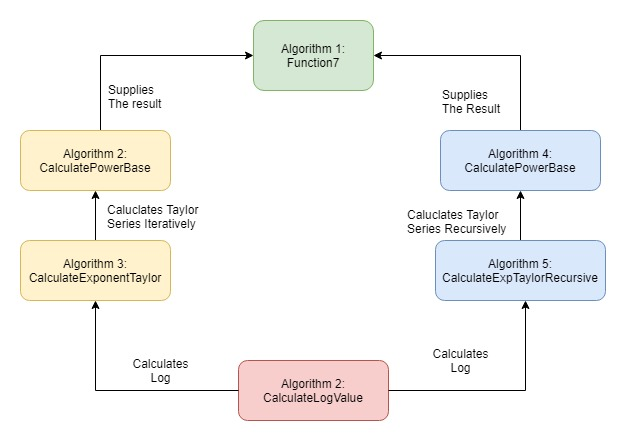
\includegraphics[width=0.61\textwidth]{Flow.jpg}
\end{figure}


\newpage
\subsection{Algorithms}
\vskip 0.198in
\begin{algorithm}
begin: \\
1. IF a,b,x are not real numbers THEN throw exception\\
2. Compute y = CalculatePower(b,x)   \\
3. z = CalculatePower(a,y) \\
4. PRINT z\\
5. REPEAT the algorithm for new value of x \\
end
\caption{Function7(a,b,x)}
\end{algorithm}
\vskip 0.198in
\begin{algorithm}
begin:\\
1. SET e = 2.718281828\\
2. SET LogOfBase = CalculateLog(base)/ CaluclateLog(e) \\
3. IF exponent $\geq$ 0 THEN\\
4. \hspace{3em} SET exponent = exponent * LogOfBase \\
5. ELSE \\
6. \hspace{3em} exponent = exponent * (-LogOfBase)\\
7. SET Result = CalculateExponentTaylor(exponent) \\
8. RETURN Result\\
end
\caption{CalculatePower(base,exponent)}
\end{algorithm}

\begin{algorithm}
begin:\\
1. SET Temp = 1 \\
2. SET i = 1 \\
3. SET Result = 0 \\
4. WHILE Temp $>$ 0\\
5. \hspace{3em} SET Result = Result + Temp \\
6. \hspace{3em} SET Temp = Temp * exponent \\
7. \hspace{3em} SET Temp = Temp / i \\
8. \hspace{3em} increment i\\
9. if exponent $<$ 0 THEN\\
10. \hspace{3em} SET Result = 1 / Result\\
11. RETURN Result \\
end
\caption{CalculateExponentTaylor(exponent)}
\end{algorithm}

\begin{algorithm}
begin:\\
1.  IF value = 1 or value = 0 THEN\\
2. \hspace{3em} RETURN 0\\
3. IF value == 10 THEN\\
4. \hspace{3em} RETURN 1\\
5. SET FLAG = FALSE\\
6. IF value $<$ 0 THEN\\
7. \hspace{3em} SET FLAG = TRUE \\
8. \hspace{3em} SET value = value * (-1)\\
9. SET LogValue = 2.302585092994046\\
10. SET BeforeDecimal = 0 \\
11. SET Result = 0 \\
12. SET Temp = 1 \\
13. WHILE value $>$ 0
14. \hspace{3em} SET value = value / 10 \\
15. \hspace{3em} increment BeforeDecimal \\
16. SET FractionalValue = (value - 1)/ (value + 1)\\
17. FOR i = 0 to 20\\
18. \hspace{3em} SET Result = Result + Temp / (2*i + 1)\\
19. \hspace{3em} SET Temp = Temp * FractionalValue * FractionalValue\\
20. SET Result = Result * 2 \\
21. SET FinalResult = BeforeDecimal + (Result / 2.302585092994046)\\
22. if FLAG = TRUE\\
22. \hspace{3em}FinalResult = (-1) * FinalResult\\
23. RETURN FinalResult\\
end
\caption{CalculateLog(value)}
\end{algorithm}

\begin{algorithm}
begin:\\
1. SET e = 2.718281828\\
2. SET LogOfBase = CalculateLog(base)/ CaluclateLog(e) \\
3. IF exponent $\geq$ 0\\
4. \hspace{3em} SET exponent = exponent * LogOfBase \\
5. ELSE \\
6. \hspace{3em} exponent = exponent * (-LogOfBase)\\
7. SET Result = CalculateExpTaylorRecursive(0,1,exponent,1) \\
8. IF exponent $<$ 0 THEN\\
9. \hspace{3em} Result = 1 / Result\\
10. RETURN Result\\
end
\caption{CalculatePower(base,exponent)}
\end{algorithm}

\begin{algorithm}
begin:\\
1. if Temp $<$ 0\\
2. \hspace{3em} RETURN Result \\
3. ELSE \\
4. \hspace{3em} RETURN CalculateExpTaylorRecursive(Result + Temp, \\ \hspace{7em}((Temp * Exponent)/counter),Exponent,counter++)\\
end
\caption{CalculateExpTaylorRecursive(Result,Temp,Exponent,counter)}
\end{algorithm}

\newpage
\subsection{Technical Reasons}

The upper sections stated two subordinate functions which were used in the solution of the function $a^{b^x}$

\begin{enumerate}
    \item It used Taylor series to find the exponent value because the domain of the function is set of real numbers which include decimal point numbers, because it is easier to handle integers but the point value power calculations can be effectively done by Taylor series.
    \item The implementation also used odd Taylor series to fine the log value of any number. Without Taylor Series we had to consider all the elements of numbers and construct a small database of log values.
    \item The two approaches stated are Recursive and Iterative where recursive approach is seems the logical choice but the consideration of java stack which is holds recursive calls is limited and for large values will run out of memory. So we use iterative approach which lets the JVM automatically handle the memory.
    \item Also the domain is -$\infty$ to +$\infty$ so the only and which can be handled by iterative approach.
\end{enumerate}
\textbf{Taylor series approach}\\
\textbf{Advantages}
\begin{enumerate}
    \item Easy calculation of complex mathematical functions
    \item Goes beyond solving normal arithmetic, it makes computing easy of large functions.
\end{enumerate}
\textbf{Disadvantages}
\begin{enumerate}
    \item Very time consuming to calculate the values.
    \item Recognize patterns to solve complex mathematical equations
\end{enumerate}

\begin{enumerate}
    \item Easy calculation of complex mathematical functions
    \item Goes beyond solving normal arithmetic, it makes computing easy of large functions.
\end{enumerate}
\textbf{Recursion Approach}\\ 
\textbf{Advantages}
\begin{enumerate}
    \item  Shorter Code, easier to write,read and debug
    \item  Advantageous in Parallel programming
    \item  Does not change the value of variable once its's declared
\end{enumerate}
\textbf{Disadvantage}
\begin{enumerate}
    \item  Trivial Base Case
    \item  Involves lots of variable declaration and usage of memory
    \item  Stack which holds recursive call values can fill up fast
\end{enumerate}
\newpage
\textbf{Iterative Approach}\\ 
\textbf{Advantage}
\begin{enumerate}
    \item  Easier to handle and debug and no Trivial Base Case
    \item  Very less limitation on the code
\end{enumerate}
\textbf{Disadvantage}
\begin{enumerate}
    \item  Large Code, Have to satisfy the conditions of the loops
    \item  Involves lots of variable declaration and usage of memory
    \item  Changes the value once it is declared
\end{enumerate}
\end{document}